% mnras_template.tex
%
% LaTeX template for creating an MNRAS paper
%
% v3.0 released 14 May 2015
% (version numbers match those of mnras.cls)
%
% Copyright (C) Royal Astronomical Society 2015
% Authors:
% Keith T. Smith (Royal Astronomical Society)

% Change log
%
% v3.0 May 2015
%    Renamed to match the new package name
%    Version number matches mnras.cls
%    A few minor tweaks to wording
% v1.0 September 2013
%    Beta testing only - never publicly released
%    First version: a simple (ish) template for creating an MNRAS paper

%%%%%%%%%%%%%%%%%%%%%%%%%%%%%%%%%%%%%%%%%%%%%%%%%%
% Basic setup. Most papers should leave these options alone.
\documentclass[fleqn,usenatbib]{mnras}

% MNRAS is set in Times font. If you don't have this installed (most LaTeX
% installations will be fine) or prefer the old Computer Modern fonts, comment
% out the following line
\usepackage{newtxtext,newtxmath}
% Depending on your LaTeX fonts installation, you might get better results with one of these:
%\usepackage{mathptmx}
%\usepackage{txfonts}

% Use vector fonts, so it zooms properly in on-screen viewing software
% Don't change these lines unless you know what you are doing
\usepackage[T1]{fontenc}
\usepackage{units}


% Allow "Thomas van Noord" and "Simon de Laguarde" and alike to be sorted by "N" and "L" etc. in the bibliography.
% Write the name in the bibliography as "\VAN{Noord}{Van}{van} Noord, Thomas"
\DeclareRobustCommand{\VAN}[3]{#2}
\let\VANthebibliography\thebibliography
\def\thebibliography{\DeclareRobustCommand{\VAN}[3]{##3}\VANthebibliography}
\newcommand{\kpch}{\,h^{-1}\unit{Kpc}}
\newcommand{\mpch}{\,h^{-1}\unit{Mpc}}
\newcommand{\hMpc}{\,h\unit{Mpc}^{-1}}
\newcommand{\msunh}{\,h^{-1}\unit{M_\odot}}
\newcommand{\software}[1]{{\small #1}}
\newcommand{\mpgadget}{\software{MP-Gadget}}
\newcommand{\HeII}{\ion{He}{II}}
%%%%% AUTHORS - PLACE YOUR OWN PACKAGES HERE %%%%%

% Only include extra packages if you really need them. Common packages are:

\usepackage{graphicx}	% Including figure files
\usepackage{amsmath}	% Advanced maths commands
% \usepackage{amssymb}	% Extra maths symbols

\newcommand{\asterix}{\software{ASTERIX}}
\newcommand{\spb}[1]{\textcolor{red}{[\bf SPB: #1]}}
\newcommand{\yueying}[1]{\textcolor{magenta}{[\bf YN: #1]}}
%%%%%%%%%%%%%%%%%%%%%%%%%%%%%%%%%%%%%%%%%%%%%%%%%%

%%%%% AUTHORS - PLACE YOUR OWN COMMANDS HERE %%%%%

% Please keep new commands to a minimum, and use \newcommand not \def to avoid
% overwriting existing commands. Example:
%\newcommand{\pcm}{\,cm$^{-2}$}	% per cm-squared

%%%%%%%%%%%%%%%%%%%%%%%%%%%%%%%%%%%%%%%%%%%%%%%%%%

%%%%%%%%%%%%%%%%%%% TITLE PAGE %%%%%%%%%%%%%%%%%%%

\title[ASTERIX]{Galaxy Formation at $z=15-3.5$ with the ASTERIX Simulation}

% The list of authors, and the short list which is used in the headers.
% If you need two or more lines of authors, add an extra line using \newauthor
\author[S.~Bird et al.]{
Simeon Bird,$^{1}$\thanks{E-mail: sbird@ucr.edu}
Yueying Ni,$^{2}$
Tiziana Di Matteo,$^{2}$
Rupert Croft,$^{2}$
Yu Feng,$^{3}$
and Yin Li$^{4}$
\\
% List of institutions
$^{1}$ Department of Physics \& Astronomy, University of California, Riverside, 900 University Ave., Riverside, CA 92521, USA\\
$^{2}$Department, Institution, Street Address, City Postal Code, Country\\
$^{3}$Another Department, Different Institution, Street Address, City Postal Code, Country
}

% These dates will be filled out by the publisher

% Enter the current year, for the copyright statements etc.
\pubyear{2021}

% Don't change these lines
\begin{document}
\label{firstpage}
\pagerange{\pageref{firstpage}--\pageref{lastpage}}
\maketitle

% Abstract of the paper
\begin{abstract}
XXXXXX
\end{abstract}

% Select between one and six entries from the list of approved keywords.
% Don't make up new ones.
\begin{keywords}
keyword1 -- keyword2 -- keyword3
\end{keywords}

%%%%%%%%%%%%%%%%%%%%%%%%%%%%%%%%%%%%%%%%%%%%%%%%%%

%%%%%%%%%%%%%%%%% BODY OF PAPER %%%%%%%%%%%%%%%%%%

\section{Introduction}
Simulations constantly get bigger. Here are some examples of big simulations. Our simulation is yet bigger. It is careful to simulate high redshifts more accurately than earlier simulations.

The main purpose of the simulation:
to model the high redshift universe. Needs larger boxes and different models. Upcoming galaxy surveys, JWST, DESI, Spherex.

\section{Methods}

% MP-Gadget.
\mpgadget~\citep{MPGadget2018} is a massively scalable version of the cosmological structure formation code Gadget-3 \citep{Springel:2005}. Although many of the basic algorithms are unchanged since \cite{Feng:2016}, the implementation has evolved significantly. Below we detail the main changes.

\subsection{Gravity}
The core of MP-Gadget remains a TreePM gravity solver, as in Gadget-3. Gadget-3's default particle mesh gravity solver
(used to compute long-range gravitational forces) is based on FFTW2. We have replaced this with a gravity solver based on a 2-d tile FFT library, \software{PFFT} \citep{doi:10.1137/120885887}.
This allows a more efficient decomposition of particles to different processors, significantly improving the
load and communication balance. To further simplify the book-keeping and reduce memory overhead,
we switched to using Fourier-space finite differencing of gravity forces, as used by the N-body gravity solver HACC \citep{2014arXiv1410.2805H}.
We also reduced the communication load by applying a sparse matrix compression of the local particle mesh.
In concert these changes removed the PM step as a scalability bottleneck. The size of the PM grid used in ASTERIX is $2^3\times N_\mathrm{PART} = 11000^3$.

Short-range forces, below the resolution of the particle grid, are computed using a hierarchical multipole expansion of the gravitational field, leading to a uniformly high force resolution throughout the computational volume. The accuracy of the gravitational algorithm has been increased and MP-Gadget is able to reproduce the matter power spectrum output by PKDGRAV3 \cite{Schneider:2016} to $<1\%$. \spb{Should we add the plot?} We replaced the error function smoothing of the particle mesh with a force smoothing kernel computed numerically \cite{Heitmann:2016} \spb{Is this the right citation? Should be more detail here}. The default scale for the short-range/long-range split ($A_\mathrm{smth}$ has been increased from $1.25$ to $1.5$, reducing force anisotropy from the particle-mesh grid. The maximum distance over which the short-range gravitational force is used has been increased from $4.5$ particle-mesh grid cells to $6$. This change increases the computational cost of the simulation (negligibly at this scale) yet improves force accuracy. With these settings, force accuracy as tested against an exact N-body solver is below $1\%$.\spb{Say what}

Since Gadget-3 and in BlueTides the tree structure used to compute short-range forces persists over short timesteps, to avoid the overhead of regenerating the force tree every timestep.
Particle motion is accounted for by moving tree nodes according to the average velocity of particles within each node. However, we found that this limited both accuracy and scalability, as the velocity of individual particles may deviate substantially from the average in the node. Accordingly, we rebuild the tree every timestep, and have implemented a number of optimizations in the tree build code to avoid it dominating the cost of the simulation, as described in \cite{Bird:2018}. The tree rebuild still represents an overhead, which we may partially address in future using the Hamiltonian gravity splitting technique from \cite{2020arXiv201003567S}.

We shift the positions of the particles by a random offset chosen uniformly between $0$ and $8$ particle-mesh grid cells, transparently undoing this offset before writing snapshots. This randomization of the particle positions relative to the box has no dynamic effect in a periodic box, but it avoids temporal correlations in the tree opening criterion, which can lead to pathological errors in tree node boundaries at high redshift \cite{2020arXiv201003567S}.

\subsection{Massive Neutrinos}

MP-Gadget includes a fast and accurate model for the effect of massive neutrinos on cosmological structure, following \cite{Yacine:2013, Bird:2018}. This model includes the dynamic effect of neutrinos in each timestep. The neutrino perturbation is computed, using a linear response formula, from the non-linear growth of the dark matter.
We assume a single massive neutrino species with a mass of $0.06$~eV, the minimum from neutrino oscillation experiments \citep{deSalas:2018}. Neutrinos of this mass suppress the matter power spectrum by about $7-8\%$ at
$k = 1 \hMpc$ and $z=9 - 2$ \citep{Bird:2018}.

\subsection{Initial Conditions}

% 2nd order Lagrangian perturbation theory with a single fluid
% Paired and fixed simulations
Initial conditions are generated at $z=99$ using a power spectrum generated from CLASS \cite{CLASS}, with cosmological parameters from \cite{Planck}. Uniquely for cosmological hydrodynamic simulations of this size, the initial conditions are generated using separate transfer functions for the cold dark matter and baryons \cite{Bird:2020}. This reduces the baryon fraction significantly at $z > 10$ and is the cause of the relative velocity effect which suppresses star formation in some halos \cite{Naoz:2007}. First-order Lagrangian perturbation theory \cite{Zeldovich:1970, Crocce:2006} is used to initialise particle positions and velocities. Radiation density is included in the cosmological background evolution, which can affect the matter power spectrum at the $10\%$ level during the reionization era.

\subsection{Hydrodynamics, star formation and stellar feedback}

The hydrodynamics, star formation and stellar feedback models largely follow \cite{Feng:2016}.
We use the hydrodynamics implementation described in \cite{2014MNRAS.440.1865F}.
We adopt the pressure-entropy formulation of smoothed particle hydrodynamics (pSPH) to solve the Euler equations \citep{2013MNRAS.428.2840H,2010MNRAS.405.1513R}.
The density estimator uses a quintic density kernel to reduce noise in SPH density and gradient estimation \citep{2012JCoPh.231..759P}. We incorporate an extra timestep criterion to limit the rate of change of the SPH smoothing length \cite{2020arXiv201003567S}:
\begin{equation}
    \Delta t_i = C_\mathrm{CFL} \frac{h_i}{d h_i / dt}\,.
\end{equation}
The Courant factor $C_\mathrm{CFL} = 0.15$. This criterion affects $\sim 1/10^{4}$ gas particles, and has minimal dynamic impact, but it prevents the smoothing length estimate becoming too inaccurate for inactive particles.

Star formation is implemented based on the multi-phase star formation model in \cite{2003MNRAS.339..289S}, and incorporating several effects following \cite{Vogelsberger:2013}.
Gas is allowed to cool both radiatively following \cite{1996ApJS..105...19K} and via metal cooling. We approximate the metal cooling rate by scaling a solar metallicity template according to the metallicity of gas particles, following \cite{Vogelsberger:2014}.
We model the formation of molecular hydrogen, and its effect on star formation at low metallicities,
according to the prescription by \cite{2011ApJ...729...36K}. Stars are formed with $1/4$ of the mass of a gas particle. Since we have also implemented mass return, the mass of a gas particle after forming $4$ stars may exceed zero. To prevent runaway enrichment as gas cycles between a star and gas particle, the $5$th star spawned from a gas particle contains the entire mass of the particle.

A stellar wind feedback model \citep{2010MNRAS.406..208O} is included, which assumes wind speeds proportional to the local one dimensional dark matter velocity dispersion $\sigma_\mathrm{DM}$:
\begin{equation}
v_w = \kappa_w \sigma_\mathrm{DM} \,,
\end{equation}
where $v_w$ is the wind speed. $\kappa_w$ is a dimensionless parameter, which we take to be $3.7$ following \cite{Vogelsberger:2013}.
Winds are sourced by newly formed star particles, which place gas particles within their SPH smoothing length into the wind. The total mass loading is $(v_w/ 350 \mathrm{km/s})^{-2}$ where $350$ km/s is in physical units. Once a particle is in the wind, it is hydrodynamically decoupled for the minimum of $60$ Myr or $20 \mathrm{kpc} / v_w$. Particles are also recoupled when their density drops by a factor of $10$, a condition which dominates most of the wind particles. Particles in the wind do not experience or produce pressure forces, nor may they be accreted onto a black hole. However, they do receive mass return, cool, and contribute to density estimates.
We have also fixed an unintentional feature in the version of MP-Gadget used for the BlueTides simulation, which led to all wind particles being recoupled at every simulation restart. This reduces the efficiency of feedback at high redshift, which has consequences for the galaxy stellar mass function.

We model patchy reionization with a spatially varying ultra-violet background using a semi-analytic method based on hydrodynamic simulations performed with radiative transfer \citep[for more details see][]{2013ApJ...776...81B}.
This method uses an evolved density field calculated from the initial conditions using second order Lagrangian perturbation theory to predict
the redshift at which a given spatial region will reionize.
In our fiducial reionization model, we set the mean reionization redshift at $z \sim 7.5$ based on the measurement of the optical depth from \cite{Planck}. In regions that have been reionized, we assume the UV background estimated by \cite{2020MNRAS.493.1614F}. We use the optically thin version, as the attenuating effects of reionization are included by our explicit reionization model.

\subsection{Helium Reionization}

We include a model for spatially inhomogeneous helium reionization following \cite{2020MNRAS.496.4372U}. Helium reionization begins at $z=4.4$ and finishes at $z=2.8$.
Helium reionization bubbles are placed around randomly chosen halos with mass $M_{\rm halo}\geq10^{12}$M$_{\odot}$, chosen to have a reasonable chance of hosting a quasar. Bubbles are $30$ Mpc/h across, matching the mean bubble size found in radiative transfer simulations \citep{2009ApJ...694..842M}. Inside this bubble a quasar radiation field is assumed with a spectral index of $-2$.

The model creates a split between photons with a mean free path larger than this bubble size, whose heating is handled homogeneously, and photons with a mean free path shorter than this bubble size, which instantaneously ionize the intergalactic gas. Particles are marked as ionized, and abruptly heated. Once marked they see the same homogeneous UVB as would be visible with the helium reionization model off.

Our model includes the patchiness of helium reionization and the resulting fluctuations in temperature, ionization state, and pressure smoothing. It captures the true scatter in the intergalactic medium temperature-density relation that should result from \HeII\ reionization.

\subsection{Metal return}

We include a model for the return of mass and metal to the inter-stellar medium from massive stars. The general approach follows \cite{Vogelsberger:2013, Pillepich:2018}, although the implementation is independent and we have created our own yield tables. The model treats each star particle as a single stellar population, with massive stars sampled using a Chabrier initial mass function (IMF) \cite{Chabrier:2003}. The lifetime of a star as a function of mass is looked up using a lifetime table from \cite{Portinari:1998}. The metal and mass yields from AGB stars, SnII and Sn1A are computed for all stars dying during the current timestep as a function of mass and stellar metallicity. Nine species are followed: H, He, C, N, O, Ne, Mg, Si, Fe. The total metallicity is tracked separately.

Stars with masses $1 M_\odot - 8 M_\odot$ are assumed to return via an Asymptotic Giant Branch (AGB) stage, with yields taken from \cite{Karakas:2010}, supplemented with \cite{Doherty:2014a, Doherty:2014b} for $M > 6.5 M_\odot$. Masses $8 M_\odot - 40 M_\odot$  return via SnII, with yields from \cite{Kobayashi:2006}. For $8 M_\odot < M < 13 M_\odot$, the tables do not contain data and so we use the yields for $13 M_\odot$ stars scaled by $M / (13 M_\odot)$. Sn1a yields are the W7 model of \cite{Nomoto:1997}. The main difference between our model and that of \cite{Pillepich:2018} lies in the treatment of stars with masses $8 - 13 M_\odot$, where \cite{Pillepich:2018} use a combination of the tables from \cite{Portinari:1998} and \cite{Karakas:2010}.\spb{We don't do that because I couldn't work out from their paper exactly what the reweighting involved.}

Mass and metal return is processed only when a star particle yields more than $10^{-3}$ of its initial mass in a single timestep. An SPH-like density kernel is computed for the star particle. Mass and metals are added to all gas particles within this kernel, fractionally divided weighted by gas particle volume and star particle SPH kernel. A technical difference between our model and that of \cite{Pillepich:2018} is that our SPH-based hydrodynamic solver lacks a mechanism for particle splitting. This reduces (numerical) diffusion of metals, but leads to the possibility of large mass variation in gas particles inside the most massive star forming halos. To avoid this we cap the gas particle mass after stellar return: any mass returned to a particle in excess of $4$ times the initial gas mass is assumed to be retained within the star. As most overweight gas particles quickly form stars, the fraction of gas particles affected at any one time is extremely low, $\sim 1/(5\times 10^7)$ in ASTERIX.

\subsection{Black Holes}

We model feedback from active galactic nuclei (AGN) in the same way as in the MassiveBlack I \& II simulations, using the super-massive black hole model developed in \cite{2005Natur.433..604D}.
Super-massive black holes are seeded with an initial mass of $5\times10^{5}\msunh$ in halos more massive than $5\times10^{10}\,h^{-1}\unit{M_\odot}$, while
their feedback energy is deposited in a sphere of twice the radius of the SPH smoothing kernel of the black hole.

\spb{Dynamical Friction model goes here...}

\subsection{Friends of Friends Groups}
\label{sec:fof}

We define dark matter halos primarily using the friends of friends (FOF) algorithm \cite{Davis1985}. This algorithm progressively associates each dark matter particle with its neighbours. Particles are associated when they are within the linking length, $0.2 \times$ mean dark matter particle separation ($9$ kpc/h for \asterix). We also associate gas, star and black hole particles with their nearest dark matter particle and thus its host halo.

We do not run subfind, which was difficult to scale to a simulation this size. To identify substructure we run (in post-processing) a second FOF algorithm on the stars belonging to each halo, with a shorter linking length of either $2$ or $5$ kpc/h. While this does not check for gravitational binding, it has the advantage that it is simple, efficient, and closely related to observational techniques for detecting high redshift galaxies by photometry. In practice most halos are dominated by a single large stellar group and so the stellar mass of the largest subhalo is similar to the stellar mass of the parent FOF group. However, especially during mergers, the center of mass of the subhalo may differ from that of the parent.

\subsection{Scalability}

\mpgadget's scalability has also been substantially enhanced  since \cite{Feng:2016}, by continued improvement of our hybrid parallelization strategy which uses both shared and distributed memory implemented with OpenMP and MPI respectively. The shared memory parallelization of the code has been improved to the point where \mpgadget~performs optimally with $>28 $ OpenMP ranks per MPI rank (in practice, we use $1$ MPI rank per processor socket). The use of OpenMP threads automatically reduces the amount of communication between ranks. Our main tree walking code uses dynamic load balancing, so that work is shared automatically between threads. Achieving this level of shared memory scalability required both parallelizing additional areas of the code (essentially all loops are now OpenMP parallel), and removing inter-thread contention. In service of the latter goal, we have mostly replaced the per-particle spinlocks used in \cite{Feng:2016} with atomic instructions. In most cases the atomic operations supported by OpenMP's atomic update directive and reduction clauses were sufficient. However, in some places we needed to perform a non-trivial calculation before updating some particle property. In these situations we make use of the atomic compare exchange compiler built-in\footnote{Our remaining spinlock protects modification of a 128 bit variable: we attempted an atomic implementation using the cmbxchg16b instruction but found it substantially slower than the (mostly uncontended) lock!}.

Distributed memory parallelism in MP-Gadget is achieved by dividing the particle tree into chunks of approximately equal particle number using a Peano-Hilbert curve.
We found that for a hydrodynamical simulation, work-load balancing based on the number of short-range gravitational forces became ineffective. Although the nominal work imbalance was indeed lower, the additional communication induced by splitting halos in half to balance the load made the total compute time to solution about $10\%$ longer. Accordingly, we perform the domain decomposition to balance particle number rather than work-load. We note that this is likely only true as we use one rank per socket rather than per processor, and thus have a substantially larger number of particles on a single MPI rank than is common in these types of simulations.

%In MP-Gadget, the time complexity to perform this decomposition is reduced from $O[N_p \log N_p]$ (in Gadget-3) to $O[\log N_p]$ \cite{Feng:2016}. We extensively over-decompose the domain

Since the tree is a shared memory structure rebuilt every timestep, particular care had to be taken to ensure the treebuild code scaled well with available core counts. We adopted a strategy in which each thread builds its own copy of the particle tree (used both for short-range gravity and SPH neighbour finding) on a subset of the particles. These duplicate trees are then merged together. To ensure the merge step is parallel, we over-decompose the domain decomposition to produce one topnode per OpenMP thread. Thus during the merge step each thread merges a separate topnode, ensuring minimal contention during the tree build.

%The key improvement was to replace communication during intermediate iteration steps with a final global broadcast of the top-level tree data structure.

We continue to use the \software{BigFile}\footnote{\url{http://github.com/rainwoodman/bigfile}} snapshot format, which transparently supports file-level striping and allows our IO to fully saturate Frontera's IO servers.


%The wall clock time for domain composition is reduced by $50\%$ with $10^4$ ranks.
%The local ``depth'' of the curve is regulated by the local particle density and work-load, such that the decomposition becomes naturally finer in high-density regions.
%The domains themselves are then generated by cutting the one-dimensional space-filling curve into $N_{\mathrm{cpu}}$ pieces that approximately induce the same computational work-load (as estimated by interaction counters for each
%particle), which automatically leads to a decomposition of space.

\section{Results}

In this Section we present some early results from the simulation, compare them to existing observations and make predictions for future higher redshift data from JWST.

\subsection{Galaxy Stellar Mass Function}

The galaxy stellar mass function, a histogram of stellar masses per unit volume, is one of the most fundamental quantities of galaxy formaton theory. However, observations do not measure it directly, but deduce it from a combination of light curves and stellar population modelling. Theoretically, it is necessary to define the boundaries of each galaxy within dark matter halos.

Figure~\ref{fig:GSMF} shows our results at $z=7 - 4$, compared to a compendium of observational data. We use the FOF routines described in Section~\ref{sec:fof} to identify galaxies. We show the GSMF computed using stars within FOF halos, but we have confirmed that it is extremely similar using subhalo stellar masses: at these redshifts, most galaxy masses are dominated by a single large component.

\begin{figure*}
\centering
  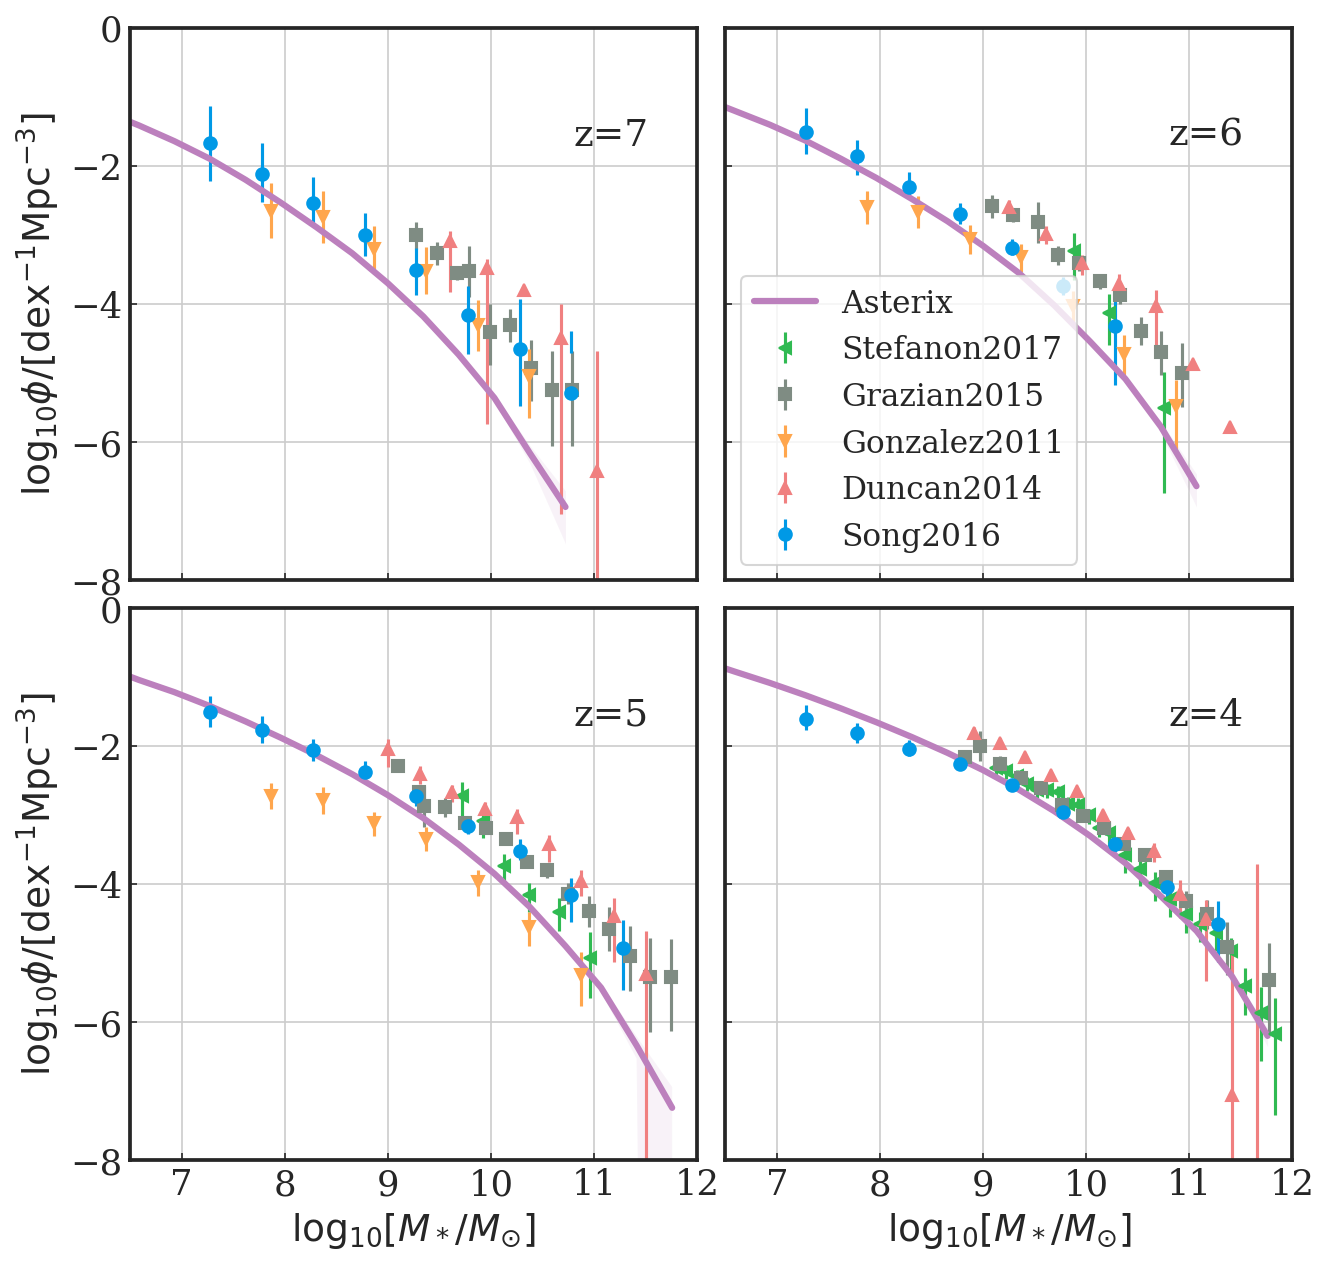
\includegraphics[width=0.8\textwidth]{plots/GSMF-z7-z4.png}
  \caption{Galaxy stellar mass functions from \asterix~for $z=7-4$. Observational data collected from \citet{Gonzalez2011}, \citet{Duncan2014}, \citet{Grazian2015}, \citet{Song2016}, and \citet{Stefanon2017}.}
  \label{fig:GSMF}
\end{figure*}

Figure~\ref{fig:GSMF} compares to observational measurements of the GSMF. At $z=4$ all datasets are in good agreement and \asterix is in good agreement, except for a mild over-production of galaxies with $M_* < 10^8 M_\odot$, which are only detected in one survey.
At higher redshift, \asterix appears to produce moderately fewer galaxies with $M_* > 9.5 M_\odot$ than observed. There is considerable scatter between different observations, reflecting the difficulty of the measurement at these high redshifts. For example, at $z=6$, the \asterix~GSMF is in good agreement with the results of \cite{Stefanon2017}, \cite{Gonzalez2011} and \cite{Song2016}, but in tension with \cite{Grazian2015} and \cite{Duncan2014}. At $z=7$, the \asterix~GSMF is lower for $M_* > 10^9 M_\odot$ than the midpoints of all measurements, although given the size of the error bars (and strong correlation between mass bins) the discrepancy is not particularly significant. Figure~\ref{fig:GSMFhighz} shows that at $z=8$, \asterix~is in good agreement with the GSMF from \cite{Song2016}, the only measurement available at this redshift.

Overall, our conclusion from the observational comparison of Figure~\ref{fig:GSMF} is that \asterix~may be producing somewhat fewer stars than observed at $z\geq 4$, but that confirmation requires improved data, perhaps from the COSMOS-Webb survey to be performed on JWST \cite{Cosmos-Webb}. Possible explanations can be found either in the simulation or in the observations. In the simulation, the GSMF at these redshifts and masses is controlled mostly by the stellar feedback. Using a test simulation with a $25$ Mpc/h box, and $550^3$ particles (thus the same mass resolution as \asterix), we found that immediately recoupling stellar wind particles to the gas (ie, allowing them to experience hydrodynamic forces), produced an increase in the GSMF which brought it into agreement with observations. At lower redshift, this model was untenable, producing substantially more stars than observed by $z=2.5$. However, a possibility is that before the completion of reionization at $5 \leq z \leq 6$, stellar feedback operates in a different, less efficient mode.

\subsubsection{Aperture and Blending}

We have also investigated the possible impact of finite photometric aperture and galaxy source blending due to redshift errors on the GSMF.

TBD.

\subsection{UV Luminosity Function}

\begin{figure*}
\centering
  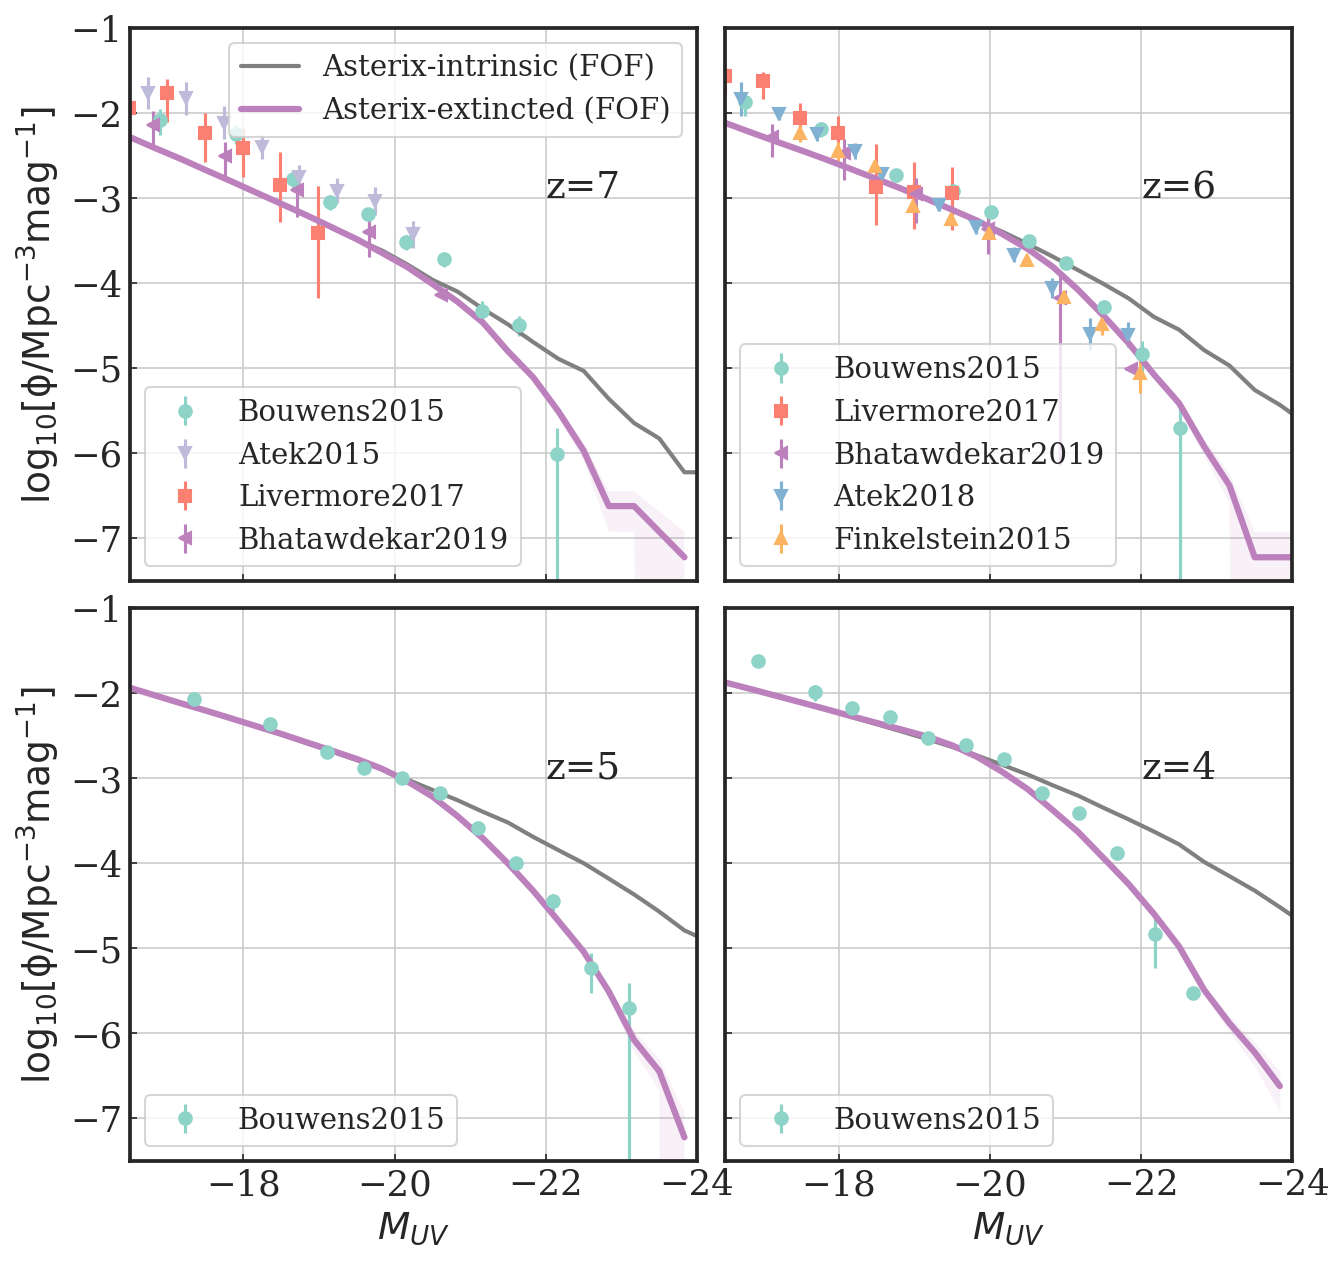
\includegraphics[width=0.8\textwidth]{plots/UVLF-z7-z4.png}
  \caption{Galaxy UV luminosity function. Data points with error bar give the current observational results collected from \citet{Bouwens2015,Livermore2017,Atek2015,Atek2018,Finkelstein2015,Bhatawdekar2019}
  \yueying{Need to do analysis based on subhalo?} \yueying{More observation data to be collected at z=5 and z=4.}}
  \label{fig:UVLF}
\end{figure*}


\subsection{Star Formation Rates}

\begin{figure*}
\centering
  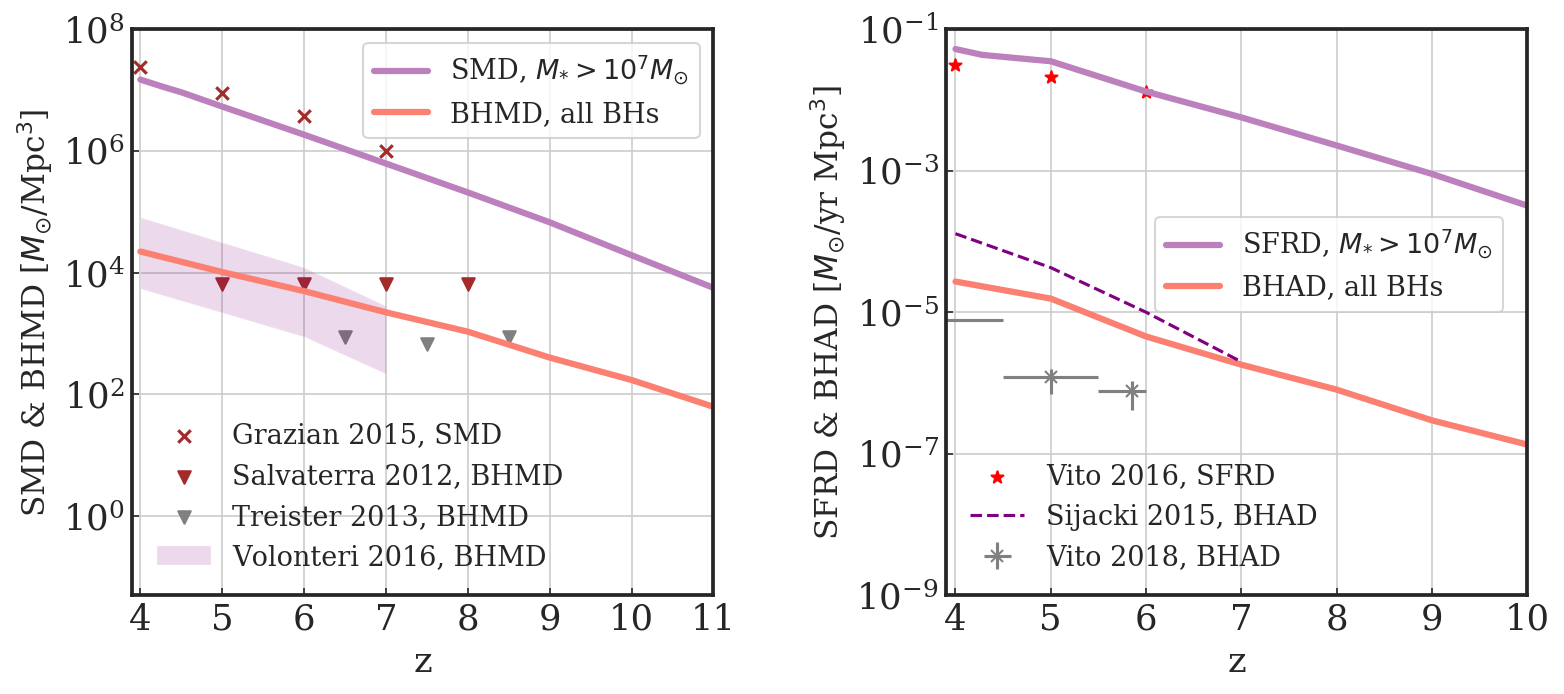
\includegraphics[width=0.9\textwidth]{plots/Global-density-hist.png}
  \caption{\textit{Left panel}: the stellar mass and BH mass density (SMD and BHMD).
  The purple solid curve show the SMD accounting for galaxies with stellar mass $M_{*} > 10^7 M_{\odot}$ in the simulation.
  The red cross give the observational result from \citet{Grazian2015}.
  The blue solid curve show BHMD for all the BHs in Asterix.
  The purple shaded area is the result from \citet{Volonteri2016}.
  The brown gray triangles are upper limits infered from the X-ray observations \citet{Salvaterra2012,Treister2013}.
  \textit{Right panel}:the SFR and BH accretion rate density (SFRD and BHAD).
  The same thresholds are used as the left panel. Observational results from \citet{Vito2016} and \citet{Vito2018} for SFRD and BHAD are shown in the brown stars and grey error bars respectively). The purple dashed line show the simulation prediction from \citet{Sijacki2015} for comparison. \yueying{Updated observation data need to be collected.}}
  \label{fig:Global-density}
\end{figure*}

\subsection{Reionization History}

\section{Conclusions}


\section*{Acknowledgements}

SB was supported by NSF grant AST-1817256.

%%%%%%%%%%%%%%%%%%%%%%%%%%%%%%%%%%%%%%%%%%%%%%%%%%
\section*{Data Availability}

The code to reproduce the simulation is available at \url{https://github.com/MP-Gadget/MP-Gadget}. \spb{Do we make halo catalogues etc public? I would think we cannot make the particle tables available...}

% Reference

%%%%%%%%%%%%%%%%%%%% REFERENCES %%%%%%%%%%%%%%%%%%

% The best way to enter references is to use BibTeX:

\bibliographystyle{mnras}
\bibliography{example} % if your bibtex file is called example.bib


% Alternatively you could enter them by hand, like this:
% This method is tedious and prone to error if you have lots of references
%\begin{thebibliography}{99}
%\bibitem[\protect\citeauthoryear{Author}{2012}]{Author2012}
%Author A.~N., 2013, Journal of Improbable Astronomy, 1, 1
%\bibitem[\protect\citeauthoryear{Others}{2013}]{Others2013}
%Others S., 2012, Journal of Interesting Stuff, 17, 198
%\end{thebibliography}

%%%%%%%%%%%%%%%%%%%%%%%%%%%%%%%%%%%%%%%%%%%%%%%%%%

% Don't change these lines
\bsp	% typesetting comment
\label{lastpage}
\end{document}

% End of mnras_template.tex
